

\subsection{A contract time object recognition tool chain}

Our second example is a more complete perception tool chain shown in Fig.~\ref{fig:chain}.
\begin{figure}[t]
	\centering
	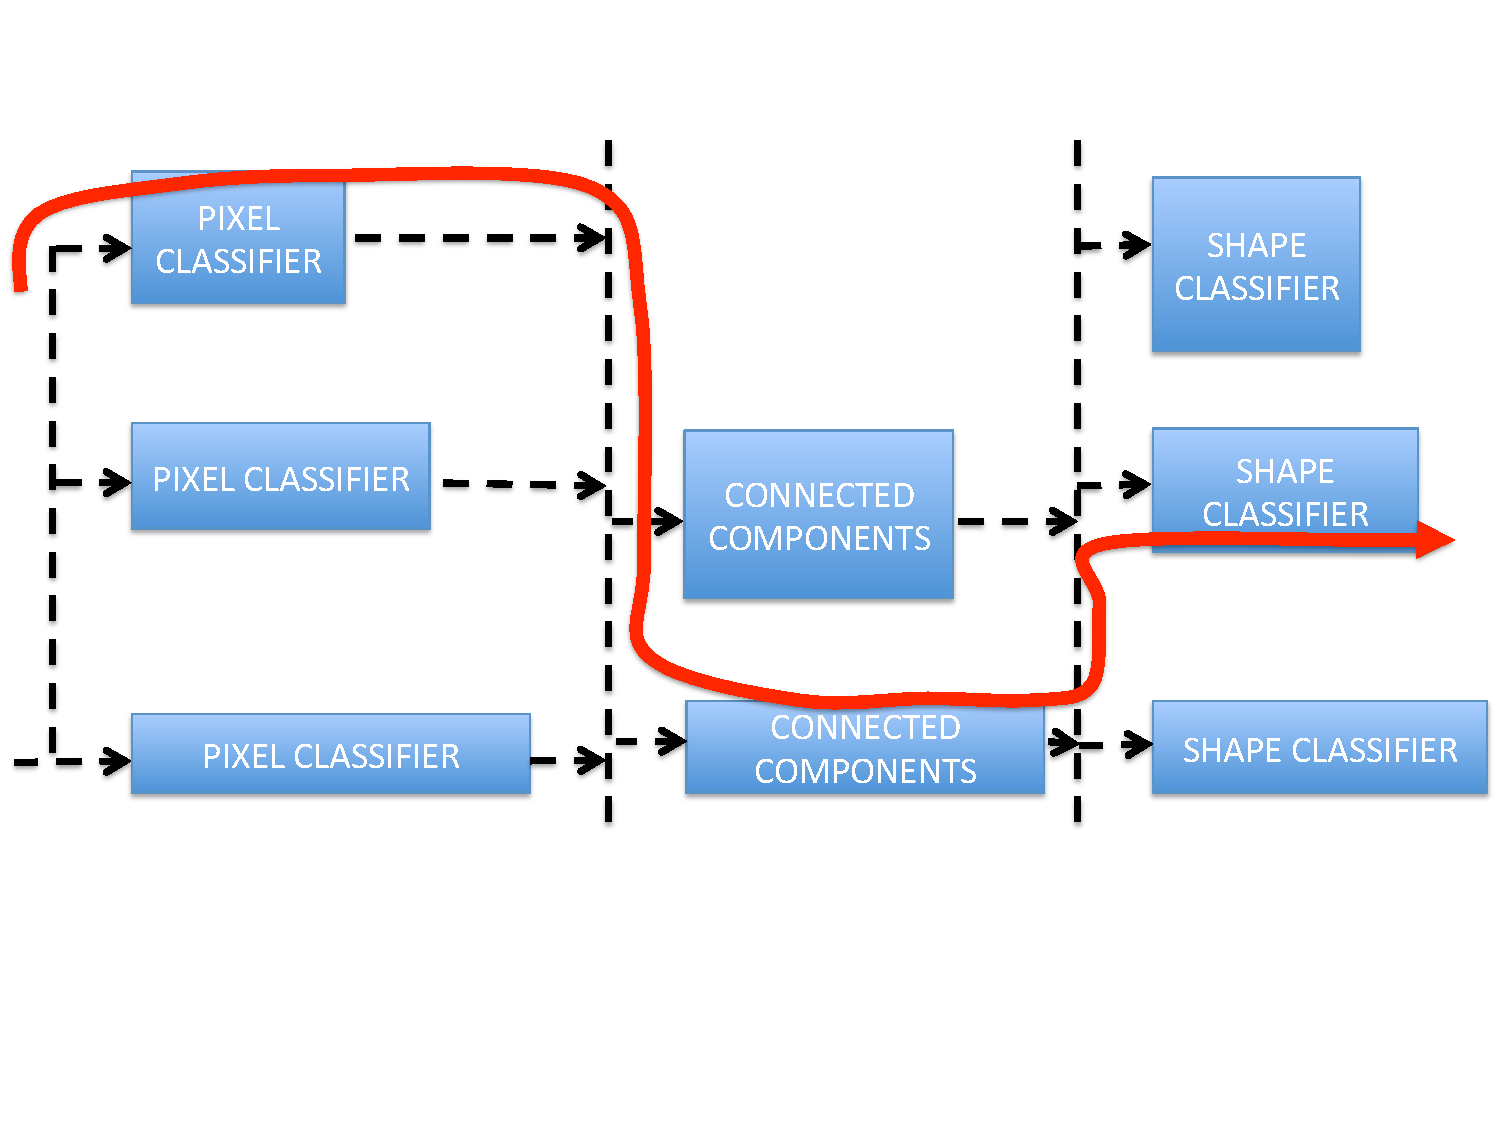
\includegraphics[width=0.9\columnwidth]{figures/chain}
	\caption{Visual perception toolchain for object detection. The height of a block indicates output error, while width indicates runtime. The red path indicates one particular execution path which trades error for runtime at each stage.}
	\label{fig:chain}
\end{figure}
The tool chain takes in a video stream and tracks an Object Of Interest (OOI) across the frames.
The pixel classifier assigns to each pixel of the image (after potential pre-processing) the probability of its being a pixel of interest, i.e., of belonging to an OOI.
A binary image is then obtained which assigns the value 1 to pixels of interest, and 0 to all others.
A Connected Components (CC) algorithm is run on the binary image to segment its 1-valued pixels into disconnected objects.
A shape classifier is then run on each object to determine whether it is an object of interest or not.
The pixel and shape classifiers are machine learning algorithms that need to be trained on a training set before being used.
In our implementation of this chain, the specific algorithms and their knobs are as follows:
the pixel classifier is a Gaussian Mixture Model (GMMs), whose knob is the number of Gaussians in the mixture.
The connected components algorithm has a two-valued knob to choose between a 4-connected and 8-connected component implementation.
The shape classifier is also a GMM, but the knob for it is the number of shape features.
The number of Gaussian components for the shape classifier is fixed since we know in advance the number of objects in the training and test sets.
Thus the knob for the entire chain is $K$ = (\#Gaussians for pixel classifier, \#neighbors for CC, \#features for shape classifier), and has a total of $3 \times 2 \times 2 = 12$ values.
Note that for any given algorithm in the chain, the relation between knob value and quality of output is not necessarily monotonic.
Like all machine learning algorithms, it will depend on the actual data set.
The same is a fortiori true of the quality of the output of the entire chain.

Fig.~\ref{fig:chainErrorDelay} shows the \emph{perception error}-delay curve for the object detection chain.
The perception error is the difference between the estimated centroid of the OOI and the true centroid of the OOI.
If the chain fails at finding the object in the frame, we assign that frame a constant error drawn from the errors found on other frames.
Each point on the curve was obtained by training the tool chain with the associated knob value, and then running the trained tool chain on the test set to obtain the $(\delta,\epsilon)$ values.
The plotted error value is the average error over all images in the test set.
The fact that the error \emph{increases} in some points despite increasing computation time can be explained by the remark made earlier: namely that the effect of a knob value is not necessarily monotonic on quality.
Moreover, the effect of a change to one algorithm of the chain might outweigh changes to other algorithms.
This makes profiling the end-to-end tool chain all the more important.
Thus, online, the controller can ignore the modes that show a degraded performance despite a higher energy cost.

This curve can then be turned into an estimate error-delay curve by incorporating it into an estimation algorithm.
\begin{figure}[t]
	\centering
	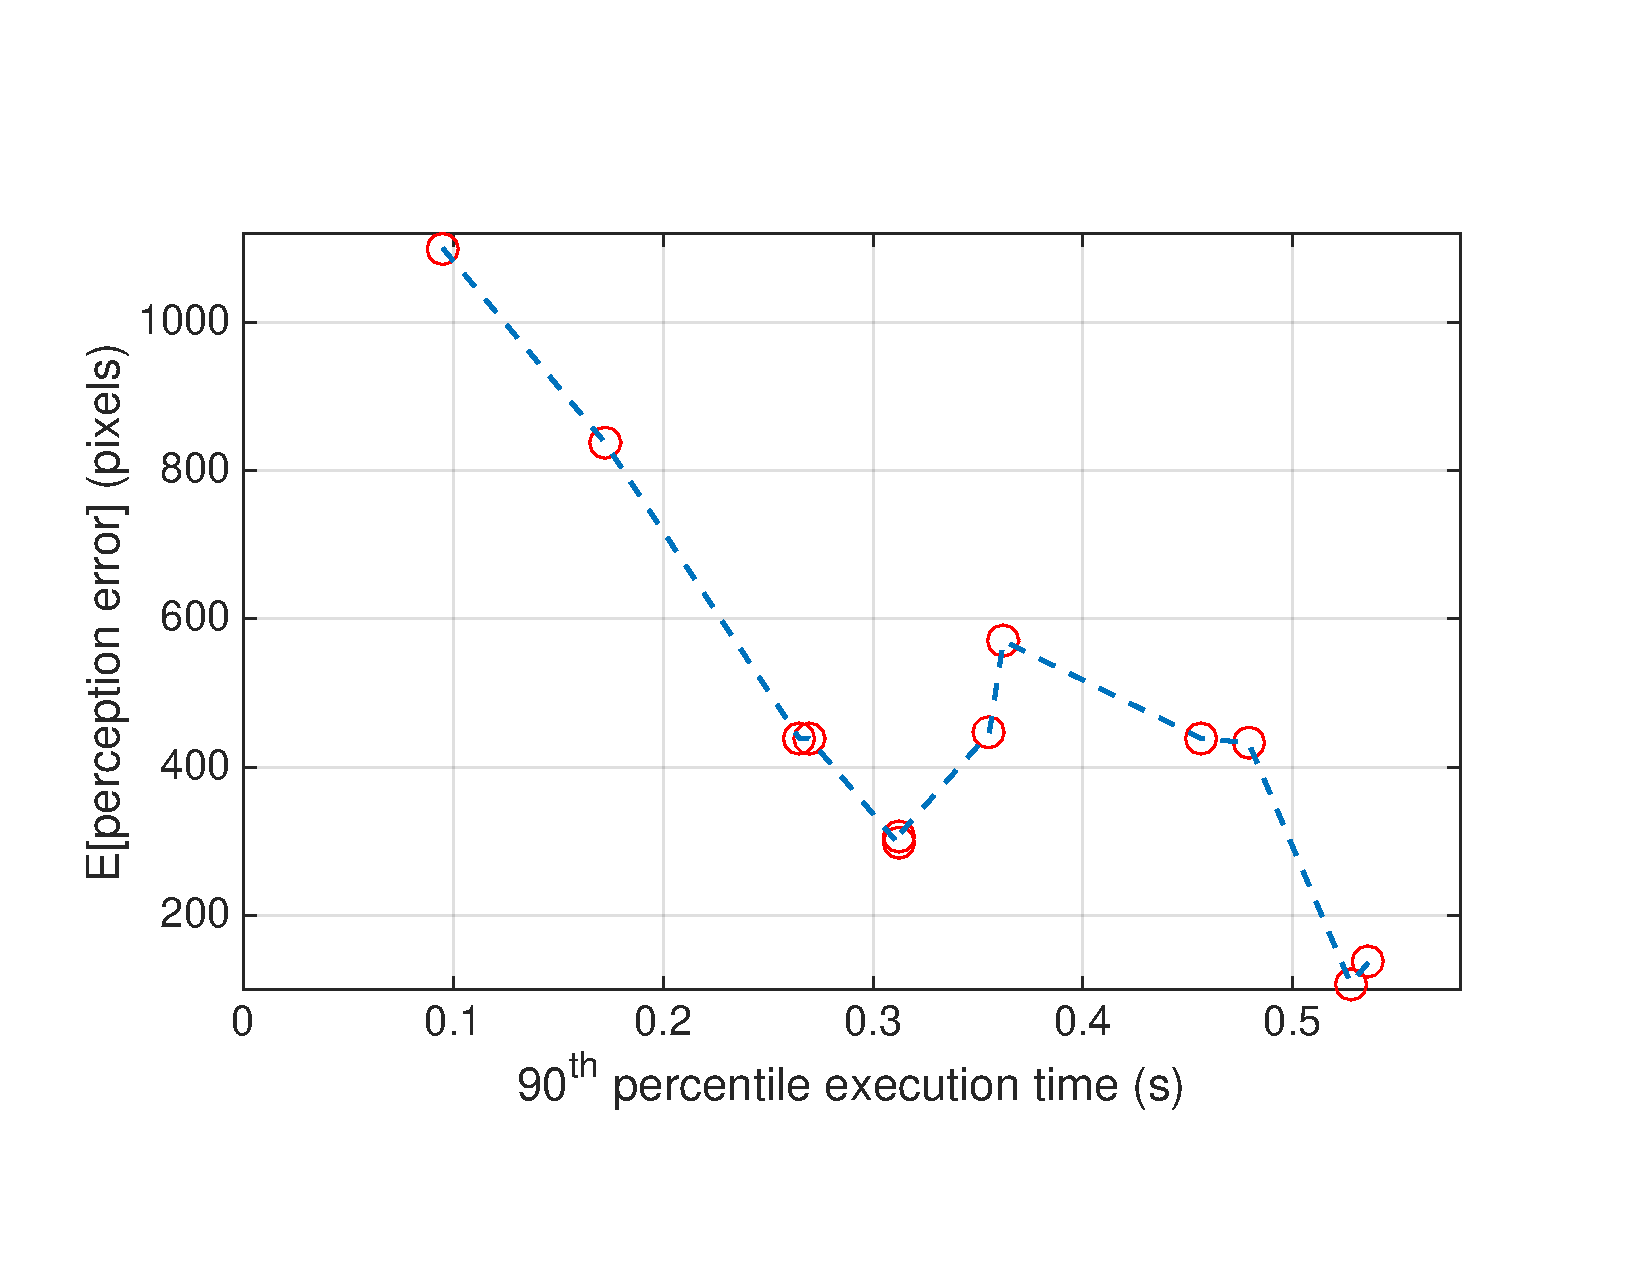
\includegraphics[width=0.9\columnwidth]{figures/chainErrorDelay}
	\caption{Perception error vs Delay curve for the chain of Fig.~\ref{fig:chain}}
	\label{fig:chainErrorDelay}
\end{figure}
More generally, such curves can be obtained for a given state estimator by identifying the knobs that control the quality and runtime of the estimator, and profiling the estimator's code at the various values of the knobs.
In effect, this gives us several Estimator tasks, each with a different utility.
I.e., each such task strikes a different balance between computation time and quality of estimate.
At time step $k$, the controller schedules the task with the best trade-off for step $k+1$, in the sense of optimizing the cost function in Eq.??

